\documentclass[11pt, spanish, a4paper, twopage]{article}
% Versión 1.er cuat 2021 Víctor Bettachini < bettachini@df.uba.ar >

% Versión 1.er cuat 2021 Víctor Bettachini < bettachini@df.uba.ar >

\usepackage[T1]{fontenc}
\usepackage[utf8]{inputenc}

\usepackage[spanish, es-tabla]{babel}
\def\spanishoptions{argentina} % Was macht dass?
% \usepackage{babelbib}
% \selectbiblanguage{spanish}
% \addto\shorthandsspanish{\spanishdeactivate{~<>}}

\usepackage{graphicx}
\graphicspath{{./figuras/}{../LaTeX/}}
% \usepackage{float}

\usepackage[arrowdel]{physics}
\newcommand{\pvec}[1]{\vec{#1}\mkern2mu\vphantom{#1}}
% \usepackage{units}
\usepackage[separate-uncertainty=true, multi-part-units=single, locale=FR]{siunitx}
\usepackage{isotope} % $\isotope[A][Z]{X}\to\isotope[A-4][Z-2]{Y}+\isotope[4][2]{\alpha}

\usepackage{tasks}
\usepackage[inline]{enumitem}
% \usepackage{enumerate}

\usepackage{hyperref}

% \usepackage{amsmath}
% \usepackage{amstext}
\usepackage{amssymb}

\usepackage{tikz}
\usepackage{tikz-dimline}
\usetikzlibrary{calc}
% \usetikzlibrary{math}
\usetikzlibrary{arrows.meta}
\usetikzlibrary{snakes}
\usetikzlibrary{decorations}
\usetikzlibrary{decorations.pathmorphing}
\usetikzlibrary{patterns}

% \usepackage[hmargin=1cm, vmargin=1cm, includeheadfoot]{geometry}
\usepackage[hmargin=1cm,vmargin=3cm, top= 0.75cm,nohead]{geometry}
% \voffset-3.5cm
% \hoffset-3cm
% \setlength{\textwidth}{17.5cm}
% \setlength{\textheight}{27cm}

\usepackage{lastpage}
\usepackage{fancyhdr}
\pagestyle{fancyplain}
\fancyhf{}
% \fancyhead{}
\setlength\headheight{28.7pt} 
\fancyhead[LE, LO]{\textbf{Física 2} (Físicos) }
% \lhead{\textbf{Física 2} (Físicos) }
\fancyhead[RE, RO]{\href{https://df.uba.ar/es/}{$\vcenter{\hbox{
\includegraphics[height=1cm]{sin_texto.pdf}}}$}}
% \rhead{$\vcenter{\hbox{
\includegraphics[height=1cm]{sin_texto.jpg}}}$}
% \rhead{
\includegraphics[height=1cm]{sin_texto.jpg}}
% \rhead{\textcopyright {\tt DF, FCEyN, UBA}}
\fancyfoot{\href{https://creativecommons.org/licenses/by-sa/4.0/deed.es/}{$\vcenter{\hbox{
\includegraphics[height=0.4cm]{cc-by-sa.pdf}}}$} \href{https://df.uba.ar/es/}{DF, FCEyN, UBA}}
% \fancyfoot{$\vcenter{\hbox{
\includegraphics[height=0.4cm]{cc-by-sa.pdf}}}$ DF, FCEyN, UBA}
% \fancyfoot{{\tiny \textcopyright DF, FCEyN, UBA}}
\fancyfoot[C]{ {\tiny Actualizado al \today} }
\fancyfoot[RO, LE]{Pág. \thepage/\pageref{LastPage}}
\renewcommand{\headrulewidth}{0pt}
\renewcommand{\footrulewidth}{0pt}


\begin{document}
\begin{center}
% \textbf{Física 2} (Físicos) \hfill \textcopyright {\tt DF, FCEyN, UBA}\\
	\textsc{\LARGE N\textgreater\textgreater1 grados de libertad}
\end{center}

Los ejercicios con (*) entrañan una dificultad adicional. Son para investigar después de resolver los demás.


\begin{enumerate}

\section*{Cadenas periódicas de N osciladores acoplados}


\item \label{anterior}
\begin{minipage}[t][1.4cm]{0.45\textwidth}
Enlazadas por resortes de coeficiente de dureza $k$ y longitud natural $l_0$ unas $N$ partículas de masa $m$ en reposo están equiespaciadas en $a$.
\end{minipage}
\begin{minipage}[c][1.4cm][t]{0.5\textwidth}
  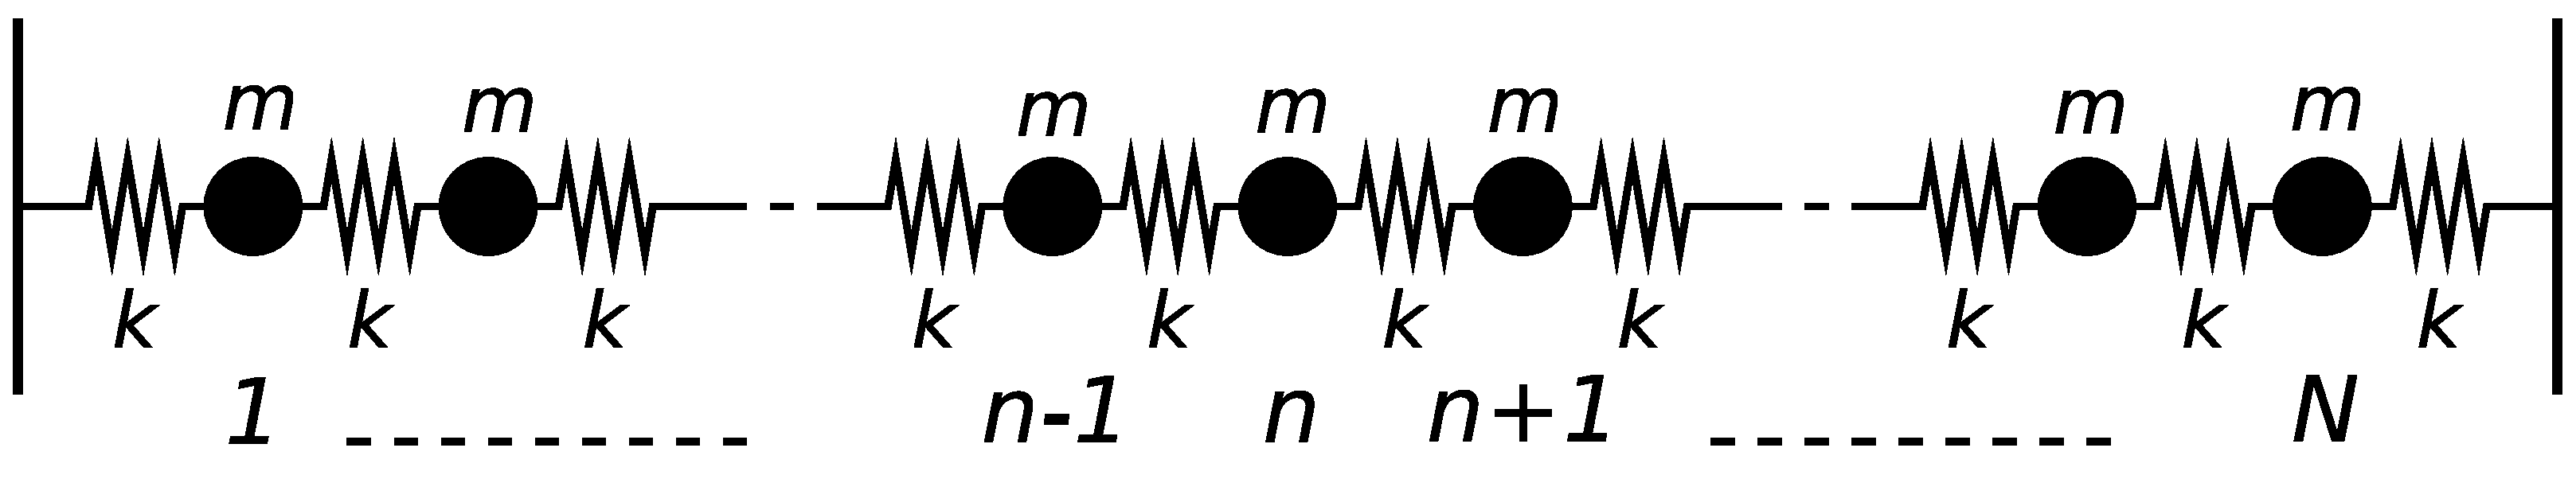
\includegraphics[width=\textwidth]{ej1-11}
\end{minipage}
\begin{enumerate}
	\item Escriba la ecuación de movimiento transversal para la partícula enésima usando la aproximación de ángulos pequeños.
	\item Se propone una solución de la forma:
	\[
		\Psi_{n}^{(p)}(t)=A^{(p)}\cos\left(nk^{(p)}a+\alpha^{(p)}\right)\cos\left(\omega^{(p)}t+\phi^{(p)}\right)
	\]
	Con ella halle la relación de dispersión.
	¿Depende esta relación de las condiciones de contorno?
	\item \label{pi} En la figura se muestra el caso de extremos fijos en que una virtual partícula $n=0$ estaría en la pared izquierda y una $n= N+1$ en la derecha.
	Escriba la solución general para la partícula enésima.
	¿Cuánto vale la frecuencia más baja?
	Haga un dibujo cualitativo del movimiento en dicho modo.
	\item \label{pa} Ídem. anterior, pero con ambos extremos están libres.
	Tal condición de contorno, a diferencia de la fija, no ejerce ninguna fuerza.
	Esto implica que la longitud de los resortes en los extremos es siempre \(a\).
	Puede modelizarse esto imponiento que \(\Psi_{n=0} = \Psi_{n=1}\) y \(\Psi_{n = N} = \Psi_{n = N+1}\).  
	\item \label{pu} (*) Ídem. anterior, pero con el extremo izquierdo libre y el derecho fijo a la pared. 
	\item (*) Particularice los resultados de \ref{pi}, \ref{pa} y \ref{pu} para el caso en que \(N = 3\).
	\item (*) Grafique cualitativamente para \(N=9\) la relación de dispersión, es decir, \(\omega^{(p)} \) en función de \(k^{(p) } \).
\end{enumerate}



\item
En el sistema de la figura hay \(N\) partículas de masa \(m\) alineadas a una distancia \(a\).
Las mismas están sujetas a las paredes mediante resortes de constante \(k\) y longitud natural \(l_0\).
A su vez, están vinculadas mediante resortes de constante también del mismo \(k\) y longitud natural \(l_0 < a\).
Hay movimiento sólo en la dirección longitudinal a las partículas.
\begin{figure}[ht]
	\centering
	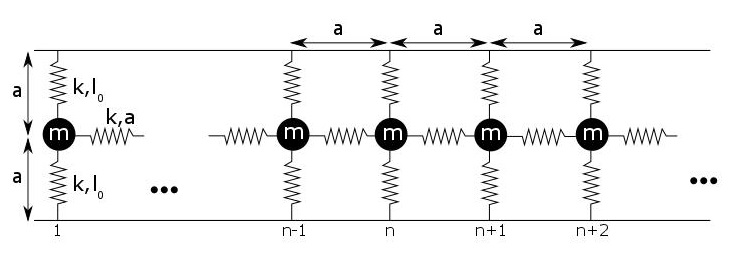
\includegraphics[width=0.7\textwidth]{g-008}
\end{figure}
\begin{enumerate}
	\item Escriba la ecuación de movimiento para la partícula énésima.
	Indique todas las aproximaciones que realiza.
	\item Proponga una solución adecuada y halle la relación de dispersión.
	¿Cuál es la frecuencia más baja posible?
	\item Imponga las condiciones de contorno apropiadas para el sistema y calcule las frecuencias propias del mismo.
	Escriba la solución para el movimiento de cada partícula.
	\item (*) Particularice para el caso \(N = 2\) y compare con el resultado que obtiene resolviendo el problema ``matricialmente''.
	Esquematice los modos normales de oscilación.	
\end{enumerate}


\item
\begin{minipage}[t][2cm]{0.6\textwidth}
 Considere el sistema de péndulos acoplados de la figura donde todos los resortes tienen longitud natural $l_0$. 
\end{minipage}
\begin{minipage}[c][2cm][t]{0.35\textwidth}
  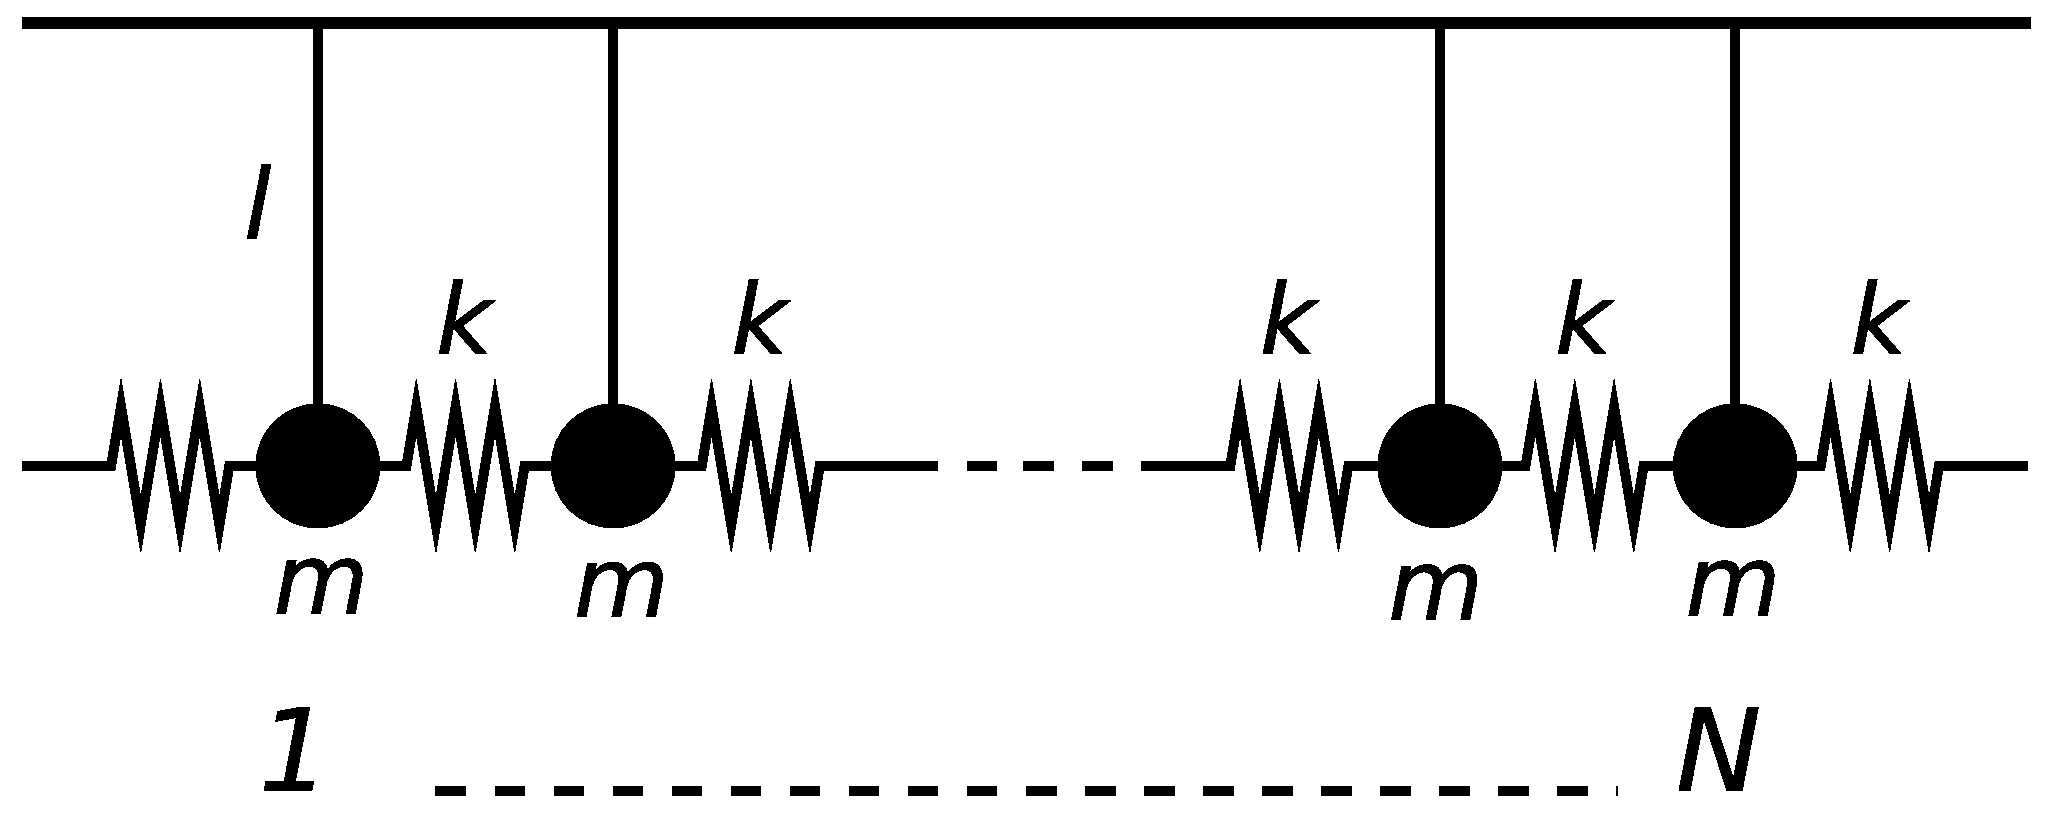
\includegraphics[width=\textwidth]{ej1-12}
\end{minipage}
\begin{enumerate}
	\item Escriba la ecuación de movimiento.
	Proponga una solución semejante a la del problema \ref{anterior} y halle la relación de dispersión.
	Compárela con la obtenida en tal problema.
	¿Cuánto vale la frecuencia más baja?
	¿Qué representa dicho modo? 
	\item Obtenga las frecuencias correspondientes a los modos normales cuando los resortes de los extremos están fijos y dé las condiciones iniciales para excitar el primer armónico. 
	\item \label{andale} Ídem anterior, pero para el caso en que uno de los resortes de los extremos está libre.
	\item 
	\begin{minipage}[t][1.6cm]{0.7\textwidth}
	(*) Particularice el problema \ref{andale} para 3 péndulos como muestra la figura.
	\end{minipage}
	\begin{minipage}[c][2cm][t]{0.2\textwidth}
  	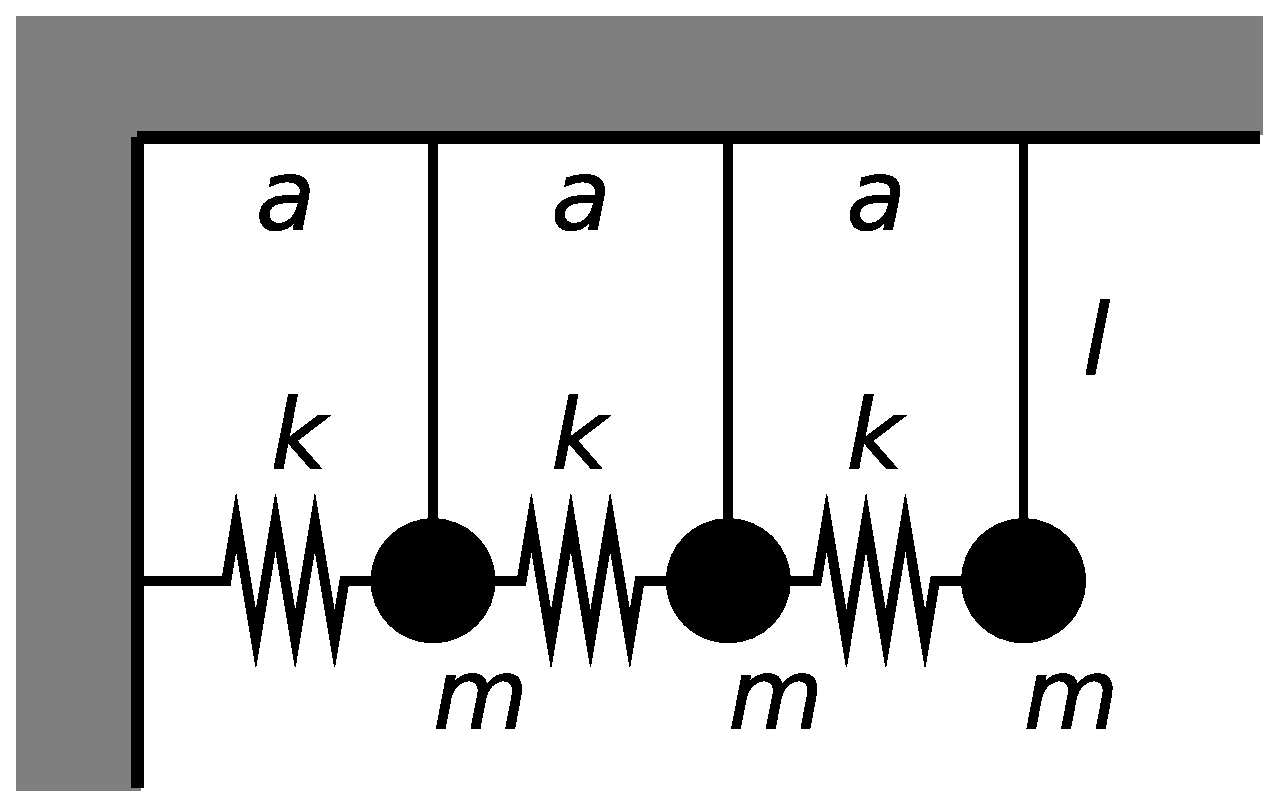
\includegraphics[width=\textwidth]{ej1-14}
	\end{minipage}
	\item (*) Suponga que en el extremo libre se aplica una fuerza \(F = F_0 \cos(\omega t)\).
	Utilizando los modos normales para el sistema sin forzar, halle la solución estacionaria del problema forzado.
	Considere el problema sin amortiguamiento.
	Utilice lo aprendido en la guía anterior.
	¿Cuáles son las frecuencias de resonancia?
\end{enumerate}


\end{enumerate}

\end{document}
